\section{Primadona-Monatip through trip}

\subsection{Overview}
Cavers undertaking the \passage[cave]{Primadona}-\passage[cave]{Monatip} through-trip will have the opportunity to complete a spectacular surface abseil, visit one of the largest chambers in the system and finish with a memorable exit panorama. \passage{Monatip} offers some challenging free-climbs and constrictions and poses some navigational problems. The trip described here starts from the \passage{Migovec Plateau} and uses the abseil rope to \passage[entrance]{Primadona} entrance. Although only 70m long, the traverse from \passage{Monatip} entrance to the surface ropes is very exposed A through trip all the way to \passage[cafe]{Sejna Soba} will take 4-6h with route finding, while the shorter round via \passage{Alkatraz} will take 3-5h. 

\subsection{Surface abseil}
The surface abseil of \passage[abseil]{Primadona} begins in a shallow valley at the USTART way point. Several rebelays on a high angle grass and scree slope lead to a lip of rock next to a prominent rock spire, which is crowned by a lightning struck bush of dwarf pine. The spire overhangs the second, more vertical part of the descent: a series of rebelays landing on various rock ledges, which eventually drop by the entrance snow slope of \passage[entrance]{Primadona}. A traverse line leading north stops short of the \passage[entrance]{Monatip} entrance, which lies just around the next rocky ridge, 70m away. Two ways into the gaping entrance of Primadona can be followed: Drugi Vhod is the high level climb into a black void, while the main route is down the snow slope.

\subsection{Entrance series to Bear Pitch}
At the bottom of the entrance snow slope (carving steps in the snow is essential to prevent a fall), a crawl over sharp cobbles, through a small drip leads to a small draughty chamber with the first pitch rope leading off. The SRT route keeps close to the western wall, a solid fault plane. After the P5, the second pitch is split in the middle by a broad, uneven ledge with many loose cobbles and boulders. It is advised to wait until the pitch is cleared by the person above before proceeding on the way out. This lands in a large 4x10m, dry, boulder strewn chamber. At the far end, a way over boulders leads to a tricky downclimb into an aven (where \passage{Drugi Vhod} comes in), while a way through the boulders leads to the top of \passage{Bear Pitch}.

\subsection{Bear Pitch to Spiral Climb}
Bear pitch is split near the top by a rebelay avoiding rub on a large ledge. The rope drops into a boulder floor chamber where a bear skeleton was discovered in the early 2000's. A carbide mark (+M) notes the place where they were found. A short traverse leads to the next drop (P15). This leads into a larger fault controlled cavern: a traverse on ledges leads to a Y-hang to reach the floor. This is followed by two short downclimbs where calcite encrusted fossils stick out of the black rock. Soon after, a window at the base of the left hand wall reveals a boulder chamber, the \passage{Spiral Climb}, but the way is in the rift, and around two massive boulders by keeping to the right hand wall in a corkscrew fashion. 

\subsection{Spiral Climb to Monatip rift - Short Route}
\textit{This short route leads directly into \passage{Alkatraz} chamber from the \passage{Spiral Climb}. After the two boulders, a climb on the right handside leads up several metres into the roof until a wriggle pops out into a small, mud floored chamber. On the far side is a steep, muddy slope descending into the western end of \passage{Alkatraz} chamber. Turning left, and going up the massive, cleanwashed boulder collapse leads to a cairned passage, the lower connection with \passage{Monatip} rift.} 

\subsection{Spiral Climb to Risanke}
Below the boulders, and under a small drip, a rift of small dimensions leads to the next pitch, with a rebelay rigged of a nose of rock protruding from the wall. At the bottom, a small downclimb passes next to water collecting bottles, and up to a dryer chamber with paper note, \passage{Lost and Found} junction.

\subsection{Risanke to Sejna Soba}
At Lost and Found junction, the way on is to the left under a rock overhang, through a constriction showing signs of blasting. A short wriggle feet first, and downclimb using the handline drops in to a boulder strewn chamber. A further pitch with a swing onto a large ledge completes the descent. From the ledge, the cairned way through the chaotic boulder collapse allows access to a larger, boulder strewn aven. Traversing over the left  of a pit leads to a narrow rift where progress is made by sideways crawling. After another smaller aven, the constrictions continue until the breakthrough into \passage{Sejna Soba}, an important nexus, recognisable due to its golden chocolate coin.

\subsection{Sejna Soba to Monatip rift}
Ducking under a rocky overhang, one can peer into the loud waterfall chamber, where a single rope leads upwards into \passage{Monatip}. \passage{Sejna Soba} is also the departure point for trips down the \passage{Galerija} and \passage{TTT} branches of the deeper \passage{Primadona}. By carefully climbing down into the chamber, and ascending the rope, one reaches an exposed traverse. By bridging along towards the NW, heedless of carbide arrows (these lead to the tight \passage{Popovezni Rov} extensions), a large aven is reached, with rope leading up and to the left. Another follows, and the top is a cramped space, with a further squeeze leading to a cairned antichamber. To the left an down the boulder slope is \passage{Alkatraz} chamber.

\subsection{Monatip rift to Planika Chamber}
Further up, the passage becomes a well traveled sinuous phreatic tube of stooping dimensions, occasionally broken by a free climb. Eventually, the passage levels out, with a wide trench in the floor leading back down. This is bypassed by a climb high into the rift which regains the original phreatic level. Further along trodden mud banks is a clean washed aven. The way on is following the source of the water, up a large pitch and into the final series of small pitches before a junction. Up to the left leads to \passage{Cloaca Maxima}, a 200m long descending crawl/stoop to the top of Alkatraz Chamber.  Up to the right, through a series of squeezes follows a strong draught until the break through at the bottom of the \passage{Monatip} \passage{Planika Chamber}.

\subsection{Big Chamber to Monatip entrance}
Climbing up the boulder slope leads to a well cairned PSS and the start of a rope. This aven was scaled and leads into the high level \passage{Monatip} extensions which eventually connect back into the east end of \passage{NCB} passage.  On the far side of the chamber, the entrance rift of \passage{Monatip} commences. From this point, the entrance is barely 6m higher in elevation, but a selection of traverses, abseils and climbs finally lead into the low, pebbly descending crawl which heralds the entrance. By keeping to the right hand passages, a small patch of grass (sometimes) dappled in sunlight heralds the end of the cave. 

\subsection{Monatip entrance to Primadona entrance}
From the entrance to \passage{Monatip}, a careful descent down the left hand side of the scree slope reaches a roped climb. This leads to a small platform overlooking \passage{Primadona} entrance over to the south, which is the start of a traverse towards the surface abseil ropes. Exposed at first  the bolted traverse soon provides a reassuring point of attachment on the thin rock ledges.

%\begin{figure*}[t!]
%\centering
%\includegraphics[height=\textheight]{curvature prima.pdf}
%\caption{ArcGIS map overlay showing 5m contours over the 10m averaged curvature}
%\label{}
%\end{figure*}

\begin{pagesurvey}
\centering
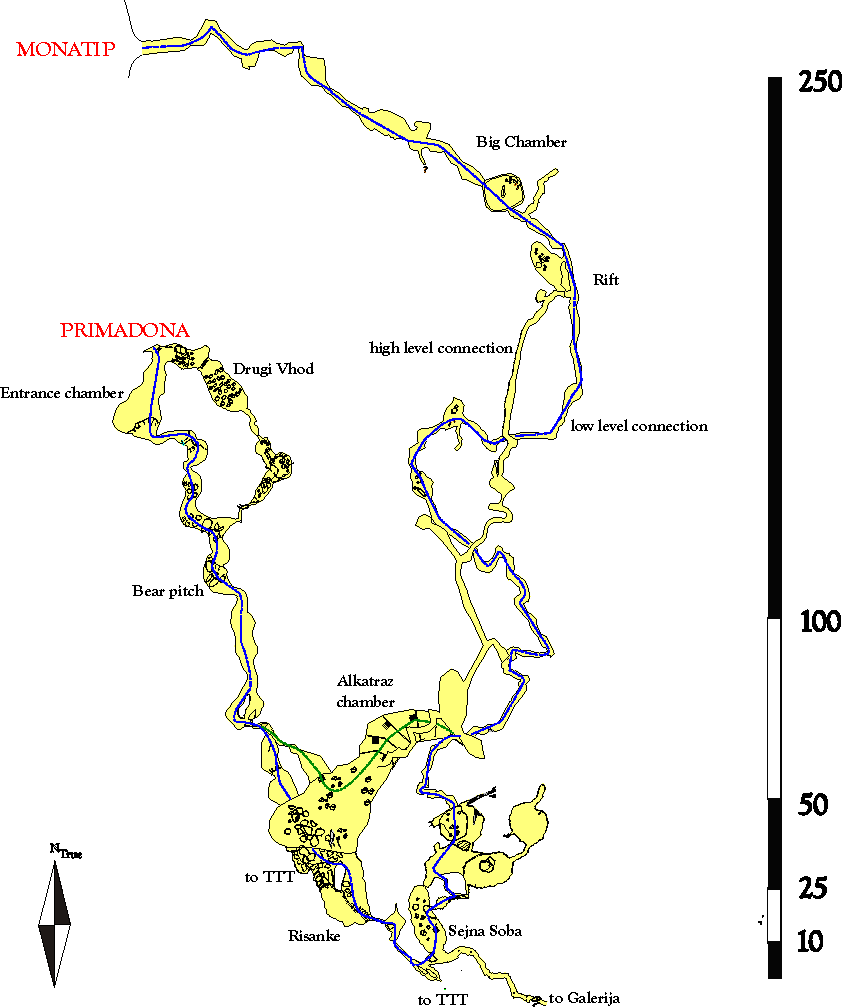
\includegraphics[height=\textheight]{images/pdf_maps/prima-mona-trip.pdf}
\caption{Plan view of the Primadona-Monatip connection passages}
\label{prima mona trip}
\end{pagesurvey}
